\chapter{Develop new analyses with Harmony}

This part explains step-by-step how to add the Harmony plug-in in your Eclipse development environment, launch harmony inside eclipse, and how to create a new analysis.


\section{Install the Harmony plug-in}
Firsts things first, you need to install Eclipse, from \url{http://www.eclipse.org/downloads/}. We recommend Eclipse Classic, as it is packaged with the Plug-in Development Environment.

Once Eclipse downloaded and unzipped, run it, and install a new plug-in via the menu \texttt{Help $\rightarrow$ Install new software}. In the "work with" field, type \url{http://se.labri.fr/data/harmony/update-site}. Select the \texttt{Harmony} category, and install the selected plug-ins.

Restart Eclipse, the harmony plug-ins are loaded in your Eclipse configuration.

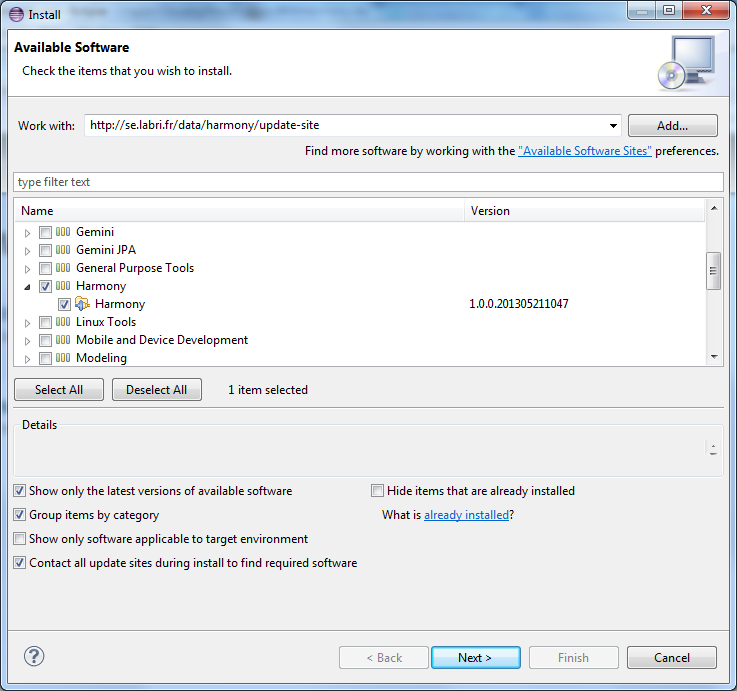
\includegraphics[width=4in]{install-harmony}

\section{Run Harmony within Eclipse}

The next step is to import the \texttt{harmony.core} plug-in in your workspace.
You can do this via the \texttt{File $\rightarrow$ Import} menu.

Then select \texttt{Plug-ins and Fragments}. In the \texttt{Import Plug-ins and Fragments} menu, select \texttt{Import As $\rightarrow$ Project with source folders}.\\

\noindent
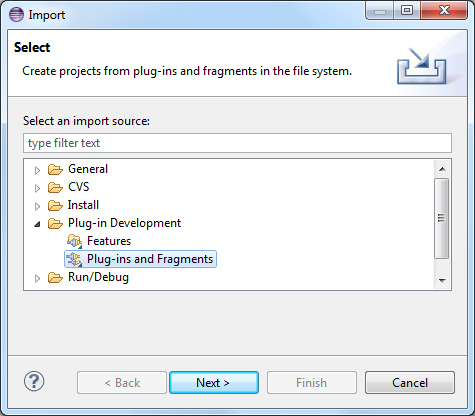
\includegraphics[width=2in]{import-menu}
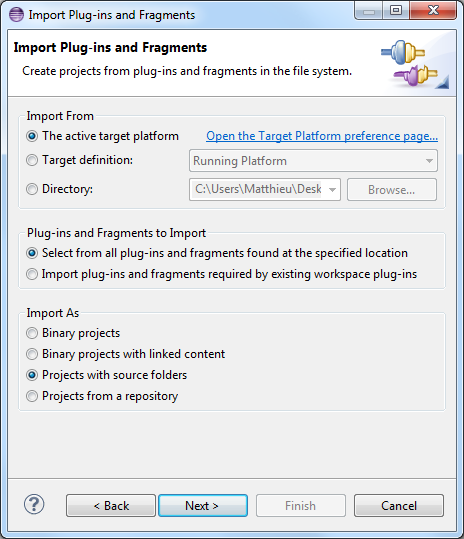
\includegraphics[width=2in]{import-plugin-menu}\\

In the next step, import the fr.labri.harmony.core plug-in.

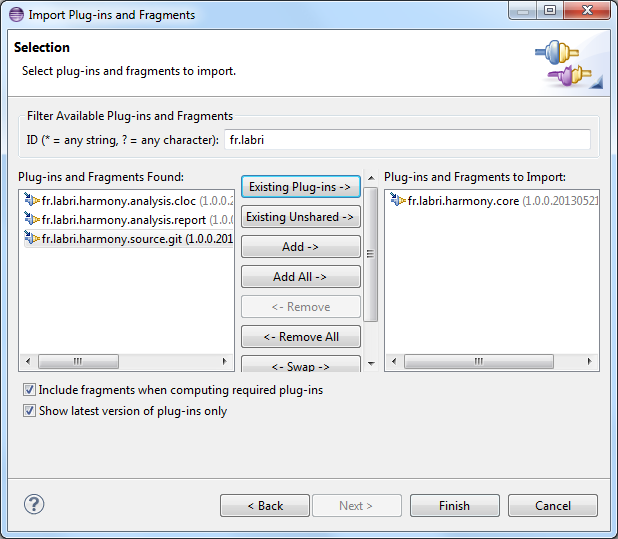
\includegraphics[width=4in]{import-plugin-selection}

Then press \texttt{Finish}; a new project has been added to your workspace.\\
You may have build errors, in such a case you need to clean the project via the \texttt{Project $\rightarrow$ Clean} menu.\\
We will be able to run Harmony in a few steps.\\
The next thing to do is to copy the configuration directory, which is inside \texttt{fr.labri.harmony.core/resources} at the root of workspace, where you should have a \texttt{.metadata} directory and the plug-in you imported:\\

\begin{lstlisting}[language=bash]
drwx------+ 1 XXXXXX None 0 21 mai   11:27 .metadata/
drwx------+ 1 XXXXXX None 0 21 mai   14:09 configuration/
drwx------+ 1 XXXXXX None 0 21 mai   13:08 fr.labri.harmony.core/
\end{lstlisting}


Then go back into Eclipse, and open the \texttt{Run Configurations} window (via the \texttt{Run} menu). In the left menu, you should see an \texttt{HarmonyEquinox} configuration under the \texttt{OSGi Framework} node. Select it.

Uncheck the "Show only Selected" checkbox (on the right), and add the harmony plugins that are not imported in your workspace (i.e. reporting, cloc, and source.git):

\noindent
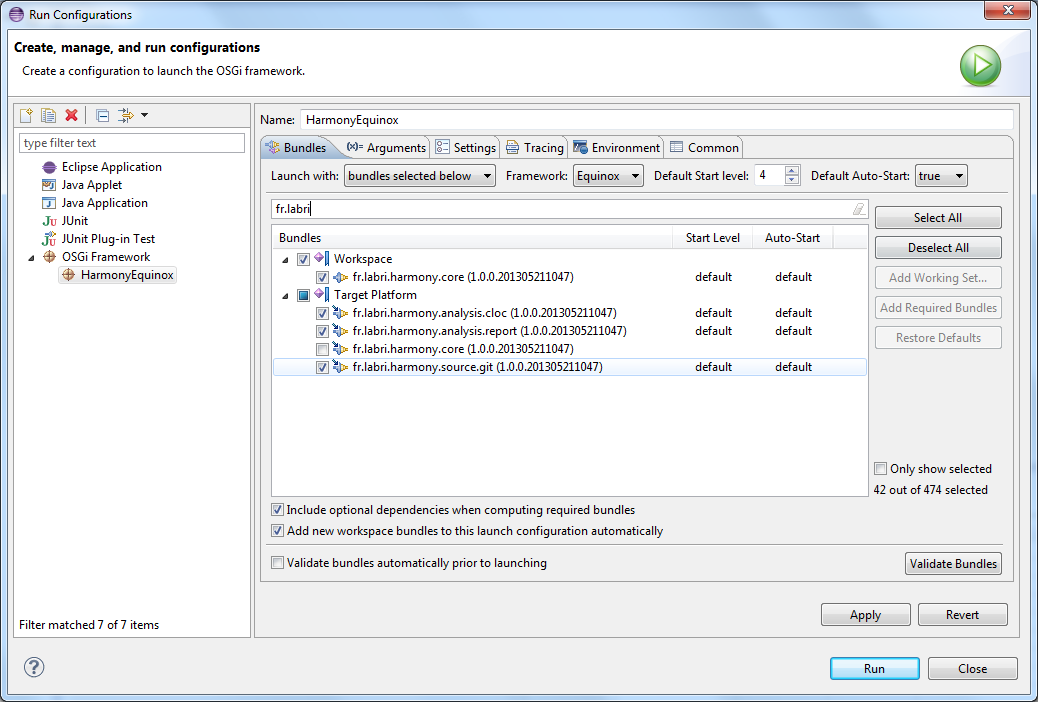
\includegraphics[width=6in]{run-configurations}

You can hit \texttt{Run}, and type \texttt{harmony} in the Eclipse console!

\noindent
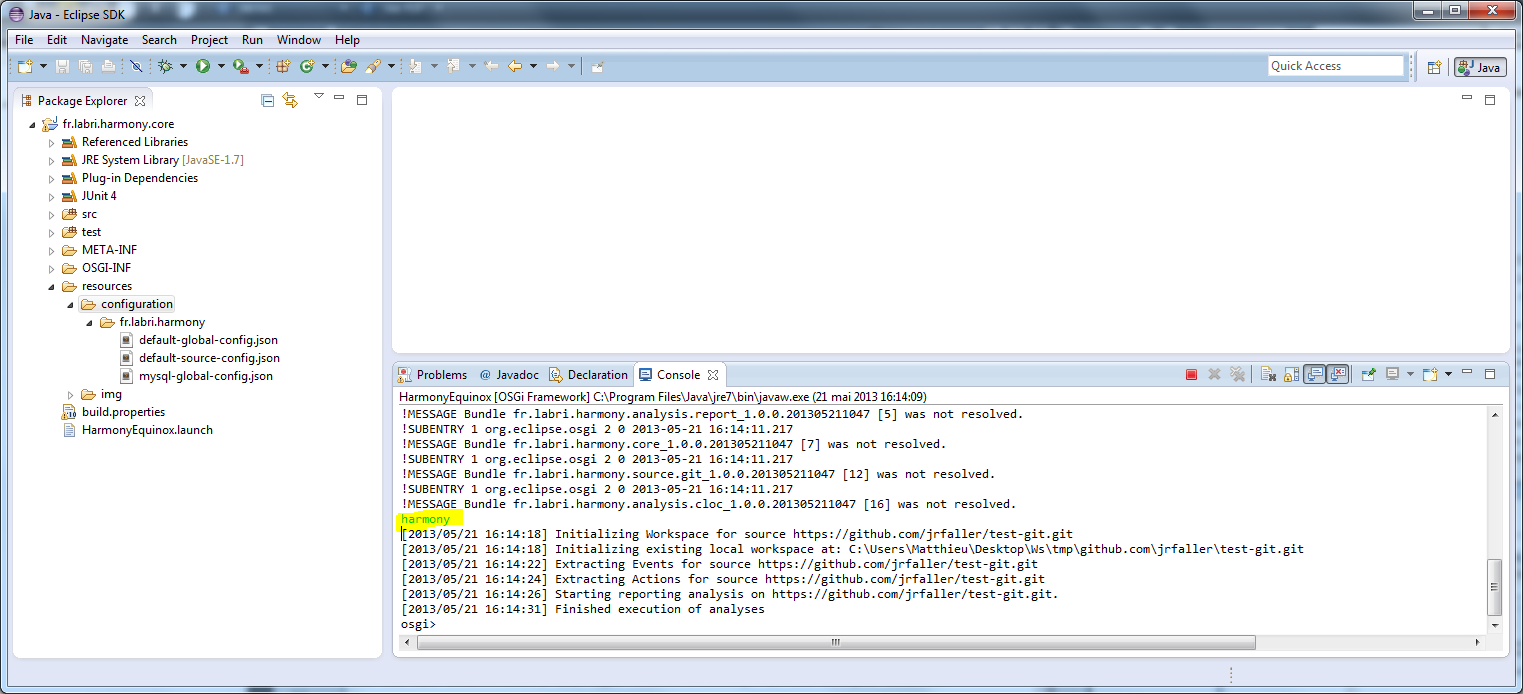
\includegraphics[width=6in]{run-harmony}

\section{Create a new analysis}

Now that Harmony can be launched inside Eclipse, we will create a new analysis.

The first step is to create a plug-in project for this analysis. We will call it \texttt{dummy}. Set the target platform to use the Equinox OSGi framework.

Press next. In the \texttt{Content} form, uncheck the \texttt{Generate an activator...} checkbox. Press next again, uncheck the \texttt{Template} checkbox, and press finish\\




\begin{center}
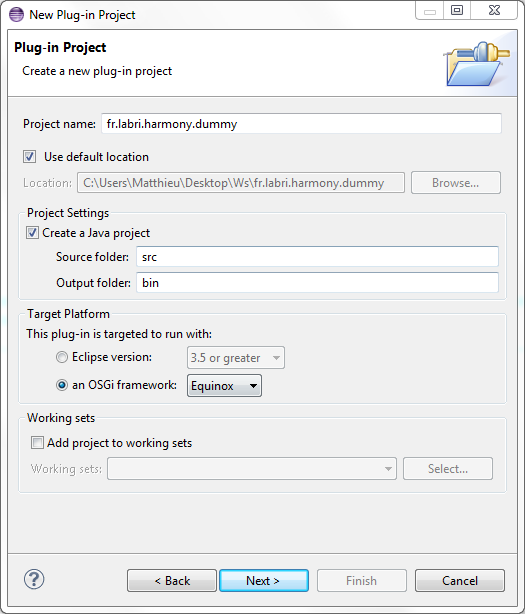
\includegraphics[width=3in]{new-plug-in}\\

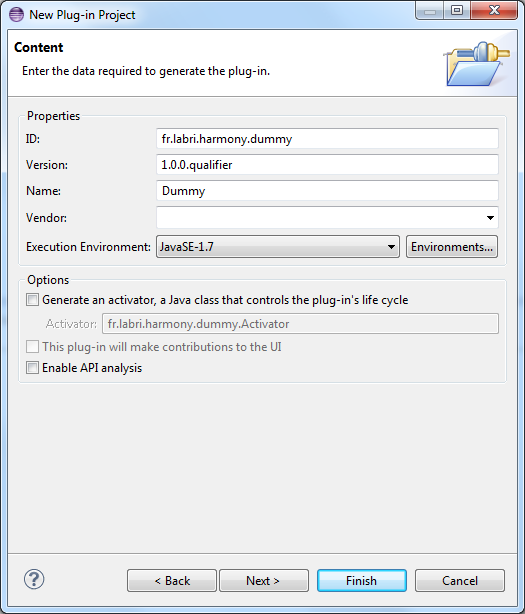
\includegraphics[width=3in]{plug-in-content}

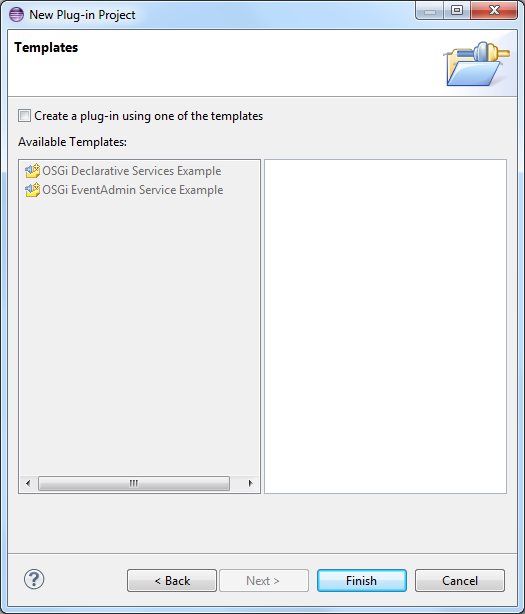
\includegraphics[width=3in]{plug-in-template}
\end{center}

In order for your analysis to use the harmony framework, you need to add the corresponding dependencies to your plug-in configuration.\\
Once you created the dummy plug-in, the \texttt{MANIFEST.MF} file should be opened in Eclipse. Open it otherwise, it is in the \texttt{META-INF} folder.\\
Open the \texttt{Dependencies} tab, and add the following imported packages:

\begin{lstlisting}
fr.labri.harmony.core
fr.labri.harmony.core.analysis
fr.labri.harmony.core.config.model
fr.labri.harmony.core.dao
fr.labri.harmony.core.log
fr.labri.harmony.core.model
javax.persistence
\end{lstlisting}

\noindent
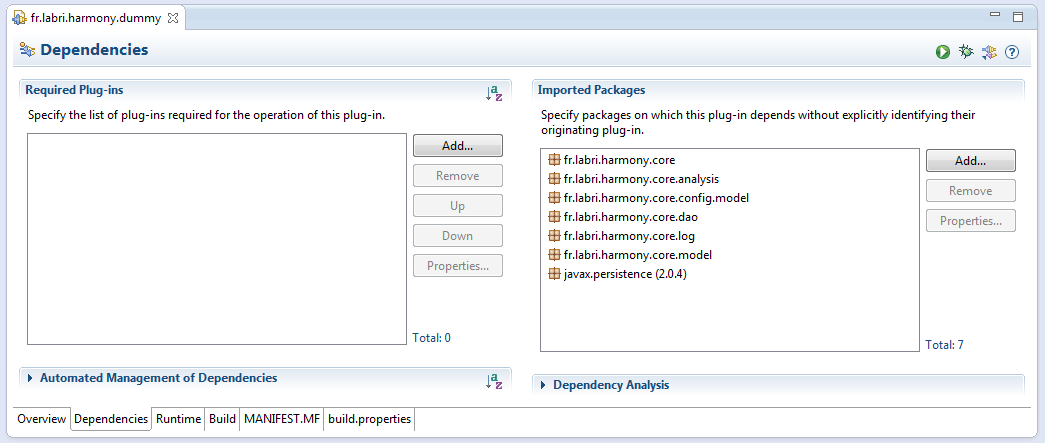
\includegraphics[width=5in]{harmony-dependencies}

Then you can add your analysis main class, which will implement the AbstractAnalysis class defined in the Harmony Core.\\
To do so, use the Eclipse \emph{new class} wizard, and check the \texttt{Constructors from superclass} checkbox. 
This is very important, as \textbf{both constructors from AbstractAnalysis are mandatory}

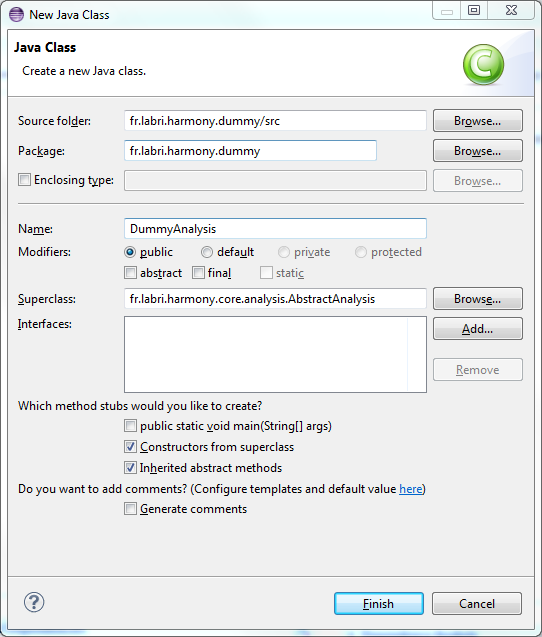
\includegraphics[width=3in]{new-java-class}

You should have the following class:



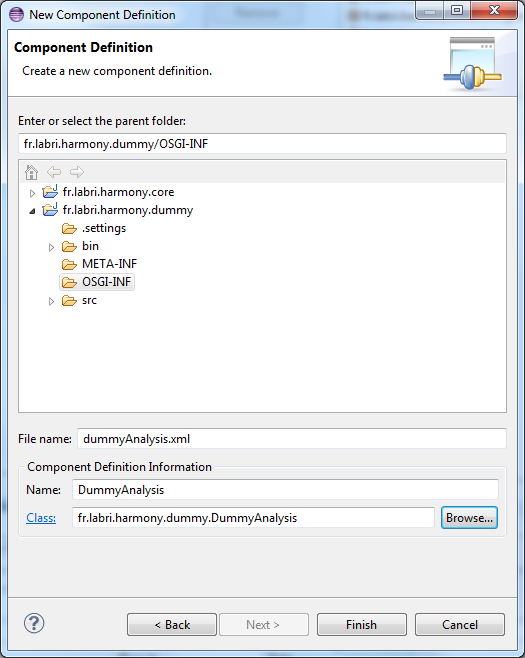
\includegraphics[width=6in]{new-component}

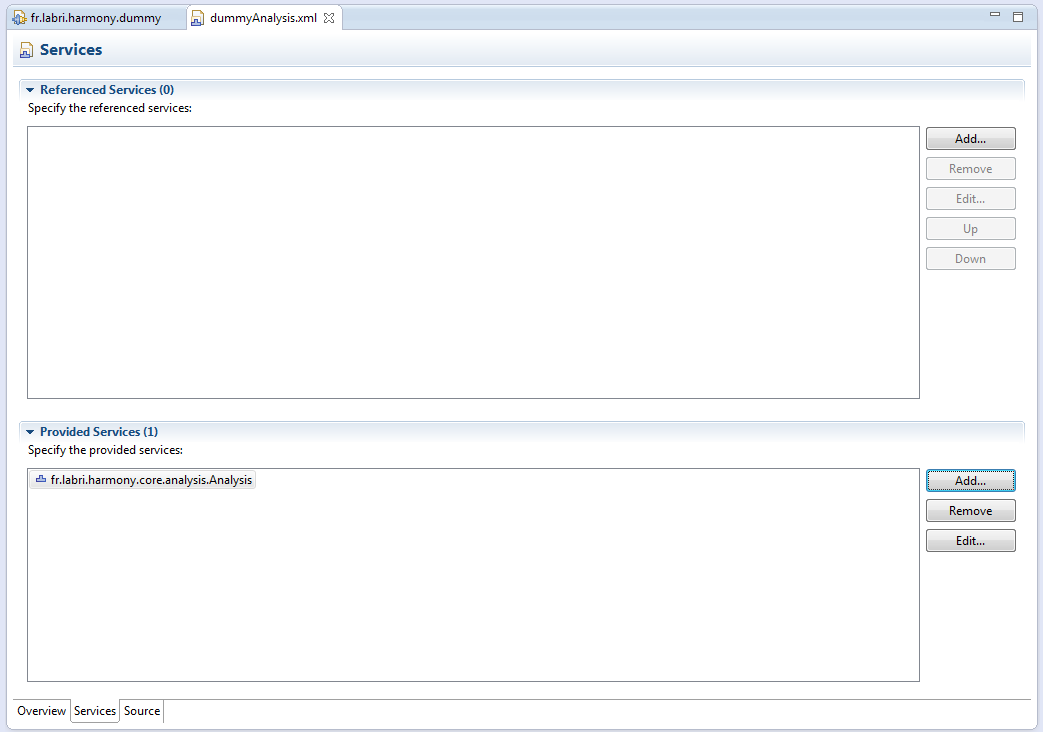
\includegraphics[width=6in]{provided-services}

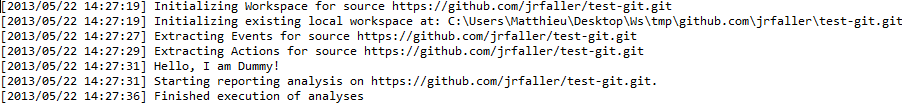
\includegraphics[width=6in]{dummy-execution}

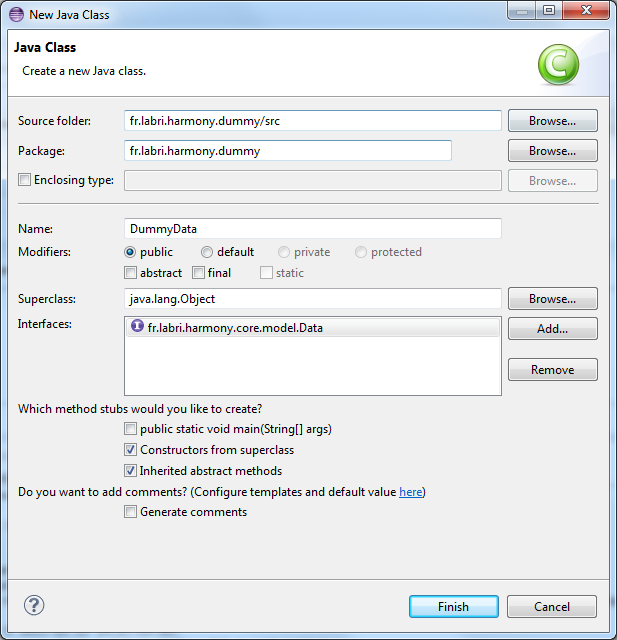
\includegraphics[width=6in]{new-data-class}


\begin{lstlisting}[language=Java]
DummyData d = new DummyData();
d.setContent("plop");
dao.saveData(this, d, Data.SOURCE, src.getId());
\end{lstlisting}




